\documentclass{standalone}
\usepackage{tikz}
\usepackage{ctex,siunitx}
\setCJKmainfont{Noto Serif CJK SC}
\usepackage{tkz-euclide}
\usepackage{amsmath}
\usetikzlibrary{patterns, calc,3d}
\usetikzlibrary {decorations.pathmorphing,decorations.pathreplacing,decorations.shapes}
\tikzset{label style/.append style={font=\small}}
\begin{document}
\small
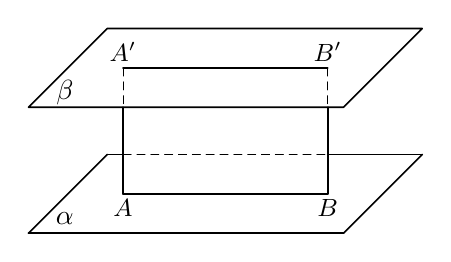
\begin{tikzpicture}[>=latex,scale=1.0,inner sep=2pt]
  \tkzDefPoints{0/0/M,4/0/N,5/1/P,1/1/Q,0/1.6/M',1.2/0.5/A,3.8/0.5/B}
  \tkzDefPointsBy[translation=from M to M'](N,P,Q,A,B){N',P',Q',A',B'}
  \tkzInterLL(A,A')(M',N')\tkzGetPoint{A1}
  \tkzInterLL(B,B')(M',N')\tkzGetPoint{B1}
  \tkzInterLL(A,A')(P,Q)\tkzGetPoint{A2}
  \tkzInterLL(B,B')(P,Q)\tkzGetPoint{B2}
  \tkzDrawPolygon[semithick](M',N',P',Q')
  \tkzDrawSegments[semithick](M,N N,P M,Q Q,A2 P,B2)
  \tkzDrawSegments[semithick](A,B A',B' A,A1 B,B1)
  \tkzDrawSegments[densely dashed](A',A1 B',B1 A2,B2)
  \tkzLabelAngle[pos=0.5](N',M',Q'){$\beta$}
  \tkzLabelAngle[pos=0.5](N,M,Q){$\alpha$}
  \tkzLabelPoints(A,B)
  \tkzLabelPoints[above](A',B')
\end{tikzpicture}
\end{document}